%    2. Write your answers in section "B" below. Precede answers for all 
%       parts of a question with the command "\question{n}{desc}" where n is
%       the question number and "desc" is a short, one-line description of 
%       the problem. There is no need to restate the problem.
%    3. If a question has multiple parts, precede the answer to part x with the
%       command "\part{x}".
%    4. If a problem asks you to design an algorithm, use the commands
%       \algorithm, \correctness, \runtime to precede your discussion of the 
%       description of the algorithm, its correctness, and its running time, respectively.
%    5. You can include graphics by using the command \includegraphics{FILENAME}
%
\documentclass[11pt]{article}
\usepackage{amsmath,amssymb,amsthm}
\usepackage{graphicx}
\usepackage[margin=1in]{geometry}
\usepackage{fancyhdr}
\usepackage{float}
\newcommand\ceil[1]{\lceil#1\rceil}
\setlength{\parindent}{0pt}
\setlength{\parskip}{5pt plus 1pt}
\setlength{\headheight}{13.6pt}
\newcommand\question[2]{\vspace{.25in}\hrule\textbf{#1}\vspace{.5em}\hrule\vspace{.10in}}
\renewcommand\part[1]{\vspace{.10in}\textbf{(#1)}}
\pagestyle{fancyplain}
\lhead{\textbf{\NAME\ (\UID)}}
\chead{\textbf{Foundations of Learning Theory}}
\rhead{CS 6966, \today}
\begin{document}\raggedright

\newcommand\NAME{Jake Pitkin}
\newcommand\UID{u0891770}
\newcommand\HWNUM{1}

\question{Problem 1}

Consider the problem of classifying points in the two-dimensional place, i.e., $\mathcal{X} = \mathbb{R}^2$. Suppose that the (unknown) true label of a point $(x, y)$ is given by sign(x) (we define sign(0) = +1, for convenience). Suppose the input distribution $\mathcal{D}$ is the uniform distribution over the unit circle centered at the origin.

\part{a} Consider the hypothesis $h$ as shown in the figure below ($h$ classifies all the points on the right of the line as +1 and all the points to the left as -1). Compute the risk $L_{\mathcal{D}}(h)$, as a function of $\theta$ (which is, as is standard, given in radians).

\fbox{ \parbox{1\linewidth}{
\begin{equation}
\setlength\fboxsep{0.25cm}
\setlength\fboxrule{0.4pt}
\boxed{Triangle \ Wave: y(\theta) = \frac{2a}{\pi} * |arcsin(sin(\frac{2\pi}{p}\theta))|}
\end{equation}

Initially I found $L_{\mathcal{D}}(h)$ to be a 2-part piecewise function dependent on the value of $\theta$. By graphing these pieces I noticed they formed a triangle wave. Using eq. 1, where $a$ is the amplitude and $p$ is the period of the wave, we can determine proper values for $a$ and $p$. An observation we can make is $L_{\mathcal{D}}(0) = 0$ and $L_{\mathcal{D}}(\pi) = 1$. Using this system of equations, we can solve for $a = 1$ and $p = 4\pi$.

	$$ L_{\mathcal{D}}(\theta) = \frac{2a}{\pi} * |arcsin(sin(\frac{2\pi}{p}\theta))| $$
	$$ L_{\mathcal{D}}(\theta) = \frac{2*1}{\pi} * |arcsin(sin(\frac{2\pi}{4\pi}\theta))| $$

\begin{equation}
\setlength\fboxsep{0.25cm}
\setlength\fboxrule{0.4pt}
\boxed{L_{\mathcal{D}}(\theta) = \frac{2}{\pi} * |arcsin(sin(\frac{\theta}{2}))|}
\end{equation}

} }


\part{b} Suppose we obtain $1/\theta$ (which is given to be an integer $\geq 2$) training samples (i.e., samples from $\mathcal{D}$, along with their true labels). What is the probability we find a point whose label is "inconsistent" with $h$? Can you bound this probability by a constant independent of $\theta$?

\fbox{ \parbox{1\linewidth}{
Let $m = 1/\theta$ where $m \geq 2$ be the number of training samples. We will consider the probability of seeing $m$ points that are \textit{all} "consistent" with a $h$ and take the compliment (being we find \textbf{a} point "inconsistent" with $h$).  \\

We know the chance of disagreement for a single training example is $L_{\mathcal{D}}(h)$, meaning the chance of agreement is given by

$$1 - L_{\mathcal{D}}(h)$$

Given the i.i.d assumption, each training example is independent. Meaning for $m$ examples we have

$$(1 - L_{\mathcal{D}}(h))^m$$

Finally, we take the compliment to get the probability we find a point inconsistent with $h$

\begin{equation}
\setlength\fboxsep{0.25cm}
\setlength\fboxrule{0.4pt}
\boxed{1 - (1 - L_{\mathcal{D}}(h))^m}
\end{equation}

To bound this probability, first we consider the values $\theta$ can take. We know $m = 1/\theta$ and $m \geq 2$ so it follows that $0 < \theta \leq 1/2$. \\ \\ We are interested in an upper bound so we will consider the valid $\theta$ with the highest $L_{\mathcal{D}}(h)$ which is $\theta = 1/2$ giving $L_{\mathcal{D}}(1/2) = 1/2\pi$ and $m = 2$. These values maximize eq. 3 for valid $\theta$ as it minimizes $(1 - L_{\mathcal{D}}(h))^m$. As $\theta$ approaches zero, $(1 - L_{\mathcal{D}}(h))^m$ approaches 1. So, letting $\theta = 1/2$ we get

$$1 - (1 - L_{\mathcal{D}}(1/2))^2$$
$$1 - (1 - \frac{1}{2\pi})^2$$
$$\frac{4\pi - 1}{4\pi^2} \approx 0.292979$$

Thus giving us an upper bound on eq. 3 given $1/\theta$ training examples and $1/\theta \geq 2$

\begin{equation}
\setlength\fboxsep{0.25cm}
\setlength\fboxrule{0.4pt}
\boxed{1 - (1 - L_{\mathcal{D}}(h))^m \leq 0.292979}
\end{equation}
} }

\question{Problem 2}

Suppose $A_1, A_2,...,A_n$ are events in a probability space.

\part{a} Suppose $Pr[A_i] = \frac{1}{2n}$ for all $i$. Then, show that the probability that none of the $A_i$'s occur is at least 1/2.

\fbox{ \parbox{1\linewidth}{
\begin{equation}
\setlength\fboxsep{0.25cm}
\setlength\fboxrule{0.4pt}
\boxed{Union \ Bound: Pr\bigg[\bigcup_{i=1}^{n} A_i\bigg] \leq \sum_{i = 1}^{n} Pr[A_i]}
\end{equation}

From eq. 3 we know that given $n$ events, the probability that at least one of those events happens is at most the sum of the probabilities of the individual $n$ events. Taking the sum of the $n$ events.

$$ \sum_{i = 1}^{n} Pr[A_i] = \sum_{i = 1}^{n} \frac{1}{2n} = n * \frac{1}{2n} = \frac{1}{2}$$

We can see that for any given $n$ events, the probability that at least one of them occurs is \textit{at most} 1/2. By showing this, we also show that the complement (none of the events occur) occurs with probability \textit{at least} 1 - 1/2 = 1/2.

$$ Pr\bigg[\bigcap_{i=1}^{n} \overline{A_i}\bigg] \geq 1/2 $$
} }


\part{b} Give a concrete example of events $A_i$ for which $Pr[A_i] = \frac{1}{n-1}$ for all $i$, and the probability that none of them occur is zero.

\fbox{ \parbox{1\linewidth}{
Let $n = 2$ giving us events $A_1$ and $A_2$ in a probability space we have

$$Pr[A_1] = Pr[A_2] = \frac{1}{n - 1} = \frac{1}{2 - 1} = 1$$
We want the probability that none of them occur, so we take the compliment of at least one of them occurring

$$Pr[A_1 \cup A_2] = 1$$
$$Pr[\overline{A_1} \cap \overline{A_2}] = 1 - Pr[A_1 \cup A_1] = 0$$

Thus showing the probability that none of them occurr is zero when $n = 2$.

} }

\part{c} Suppose $n \geq 3$, and $Pr[A_i] = \frac{1}{n -1}$, but the events are all \textit{independent}. Show that the probability that none of them occur is $\geq$ 1/8.

\fbox{ \parbox{1\linewidth}{
\begin{equation}
\setlength\fboxsep{0.25cm}
\setlength\fboxrule{0.4pt}
\boxed{Multiplication \ Rule: Pr\bigg[\bigcap_{i=1}^{n} A_i\bigg] = \prod_{i = 1}^{n} Pr[A_i]}
\end{equation}

Given the events $A_i$ are independent, we can use the multiplication rule to determine the probability they all occur. We are interested in the probability none of them occur, so we will take the compliment of each $A_i$.

\begin{align*}
Pr\bigg[\bigcap_{i=1}^{n} \overline{A_i}\bigg] &= \prod_{i = 1}^{n} 1 - Pr[A_i] \\
 &= \prod_{i = 1}^{n} 1 - \frac{1}{n-1} \\
 &= \prod_{i = 1}^{n} \frac{n - 2}{n-1} \\
 &= \bigg(\frac{n-2}{n-1}\bigg)^n
\end{align*}

We want to show for all $n \geq 3$ so we will show for $n = 3$

$$Pr\bigg[\bigcap_{i=1}^{3} \overline{A_i}\bigg] = \bigg(\frac{3-2}{3-1}\bigg)^3 = \bigg(\frac{1}{2}\bigg)^3 = \frac{1}{8}$$

We see that $n = 3$ is satisfied and we can observe the function grows as $n$ grows by looking at the ratio of $n$ and $n-1$ events

$$ \frac{(\frac{n-2}{n-1})^n}{(\frac{n-3}{n-2})^{n-1}} \geq 1 \ \ \  \forall \ n \geq 4$$

Taking the $l  i  m_{n\to\infty}$ we see that it converges to 1/$e$

$$\lim_{n\to\infty}\bigg(\frac{n - 2}{n - 1}\bigg)^n = \frac{1}{e} \approx 0.3679$$

Thus proving given $n$ independent events with $Pr[A_i] = \frac{1}{n-1}$, the probability that none of them occur is $\geq 1/8$.

} }

\question{Problem 4}

Recall that the VC dimension of a hypothesis class $\mathcal{H}$ is the size of the largest set that it can "shatter".

\part{a} Consider the task of classifying points on a 2D plane, and let $\mathcal{H}$ be the class of axis parallel rectangles (points inside the rectangles are "+" and points outside are "-"). Prove that the VC dimension of $\mathcal{H}$ is 4.

\fbox{ \parbox{1\linewidth}{
The proof that the VC dimension of $\mathcal{H}$ is 4 comes in two parts. First, we will provide a concrete example of 4 points that can be shattered by $\mathcal{H}$. This is will prove that the VC dimension of $\mathcal{H}$ is $\geq 4$. Next, we will prove that \textbf{no} set of 5 points cannot be shattered by $\mathcal{H}$. This proves that the VC dimension of $\mathcal{H}$ is $< 5$. The combination of these two bounds proves the VC dimension of $\mathcal{H}$ is 4. \newline

\textit{proof VC dimension of $\mathcal{H} \geq 4$ - } Let us consider 4 points on the 2D plane $x_1, x_2, x_3, x_4$ where these 4 points form a diamond. Given binary labeling and 4 points, there are 16 possible labelings. All of the possible labelings can be correctly captured by a axis-parallel rectangle.

\begin{figure}[H]
  \centerline{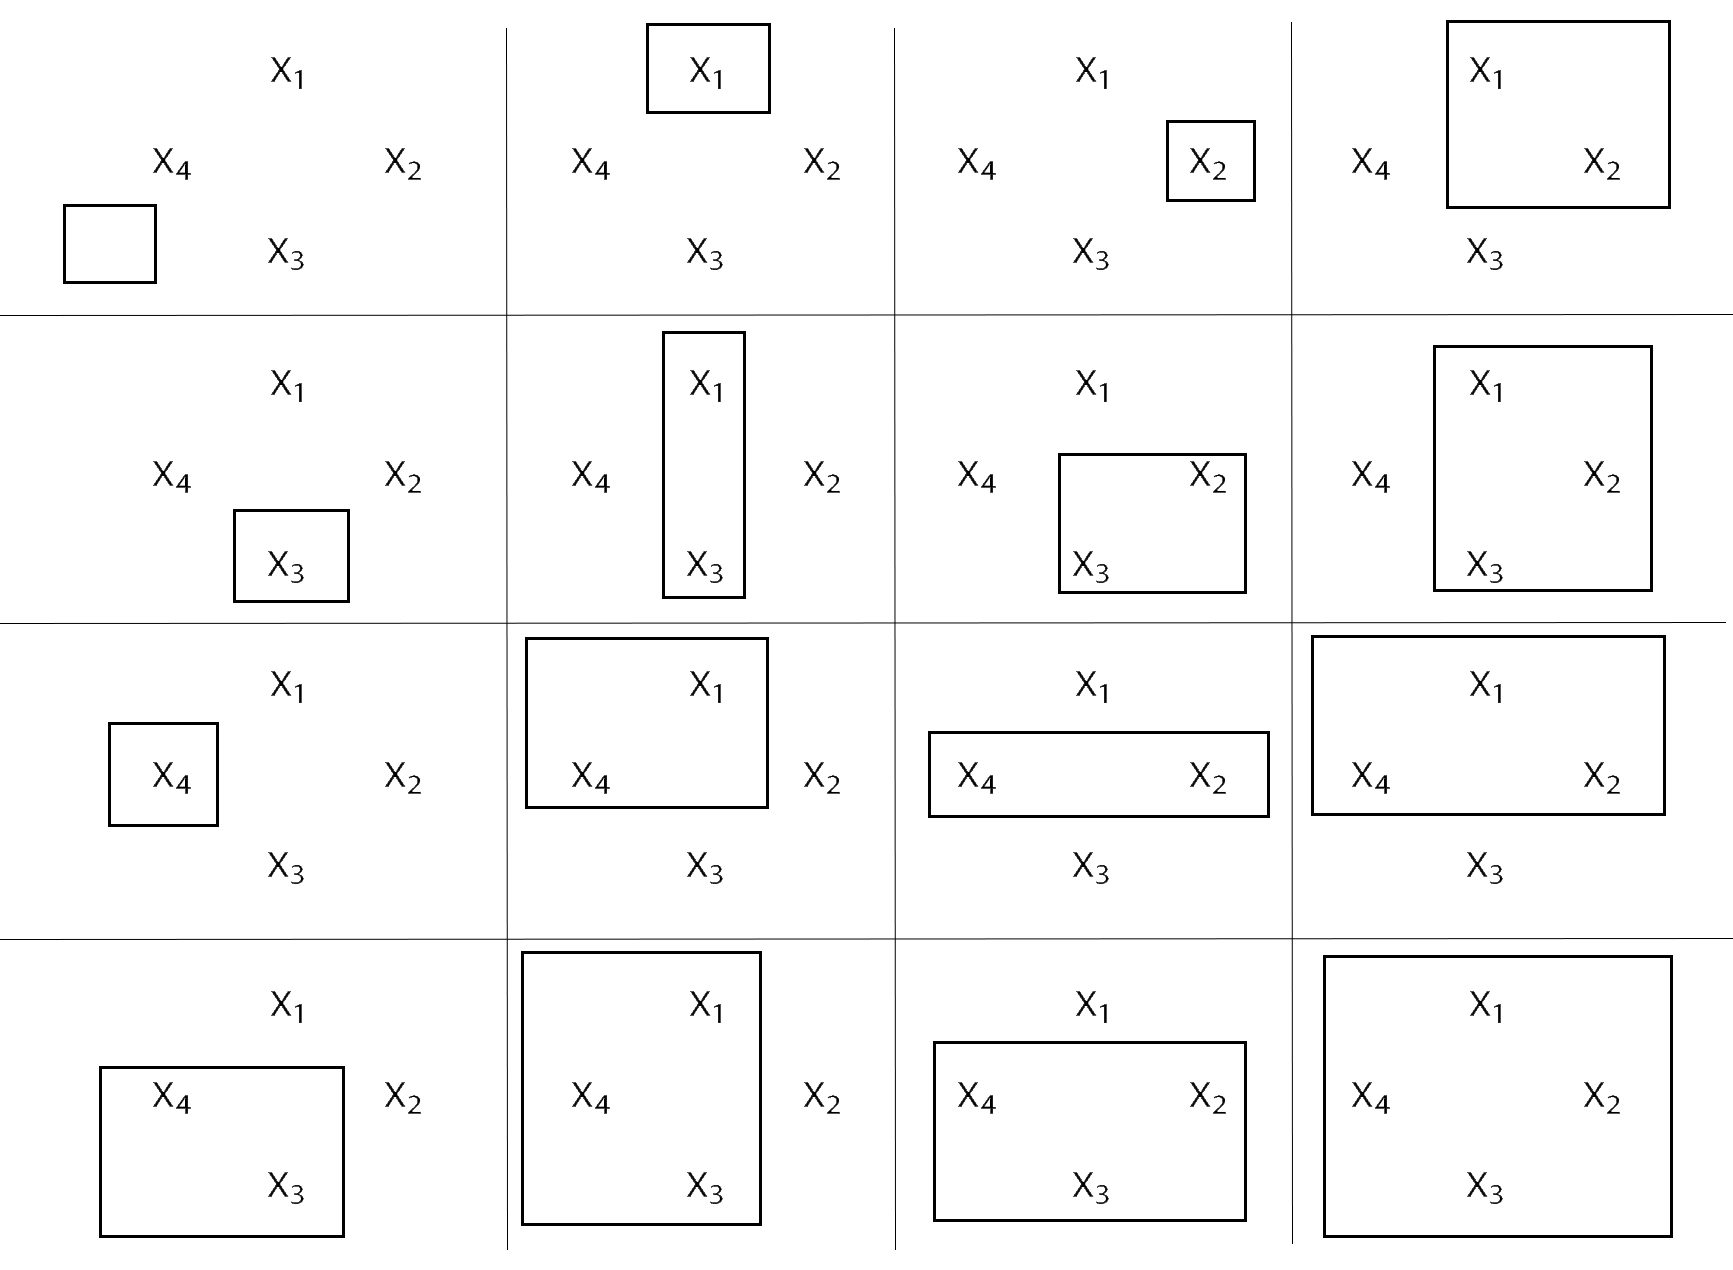
\includegraphics[width=0.8\linewidth]{4a.png}}
  \caption{All possible assignments of labels classified.}
\end{figure}
Thus proving the VC dimension of $\mathcal{H}$ is $\geq 4$. \newline

\textit{proof VC dimension of $\mathcal{H} < 5$ - } Now we consider \textbf{any} set of 5 points in the 2D plane and show that there is a labeling that cannot be captured by $\mathcal{H}$. As there exists an infinite number of possible subsets of 5 points we can't consider every subset. Rather, we will consider the different forms the 5 points can take. \newline

The 5 points can appear in a line (horizontal, vertical, or diagonal), 4 points can form a convex hull with the 5th point inside, or 4 points can form a convex hull with the 5th point outside that square. For a line, the points could adversarially labeled by alternating their labelings. Clearly an axis-parallel rectangle can't capture this. The other two formations can be labeled adversarially such that there are two regions of + labeled points with a region of - labeled points laying between them. To visualize this, consider the example of 4 points, but placing the 5th point in the middle of the diamond allowing for a "wall" to be formed between the other two points. \newline

We can conclude that VC dimension of $\mathcal{H}$ is 4 as we have proven that it is $\geq 4$ and $< 5$.

} }

\part{b} This time, let $\mathcal{X} = \mathbb{R}^d \ \backslash \ \{0\}$ (origin excluded), and let $\mathcal{H}$ be the set of all hyperplanes through the origin (points on one side are "+" and the other side are "-"). Prove that the VC dimension of $\mathcal{H}$ is $\leq d$.

\fbox{ \parbox{1\linewidth}{
\textit{proof by contradiction -} Assume that the VC dimension of $\mathcal{H}$ is $> d$. Namely, as suggested by the hint, let's assume that $\mathcal{H}$ can shatter any $d + 1$ points from $\mathcal{X}$. Denote these points as the set $\mathcal{X^\prime} = \{\mathbf{x}_1, \mathbf{x}_2, ... , \mathbf{x}_d, \mathbf{x}_{d +1}\}$. This means there must exist an $h \in \mathcal{H}$ that properly labels the d + 1 points, for every possible labeling. For this to be true, there must exist $2^{d+1}$ corresponding weight vectors $\mathbf{w}_i \in \mathbb{R}^d$ (each of which defines a $h \in \mathcal{H}$) such that

$$h(\mathbf{x}_i) = sign(\mathbf{w}^T\mathbf{x}_i)$$

produces the correct label $y_i$ for each point $\mathbf{x}_i \in \mathcal{X}^\prime$. Let $\mathbf{W} = \{\mathbf{w}_1, \mathbf{w}_2, ... ,\mathbf{w}_d, \mathbf{w}_{d+1}\}$, we can represent $\mathbf{W}\mathcal{X^\prime}$ as a matrix where each entry is the sign of the cross product $a_{i,j} = w_i^Tx_j$.

$$A = \begin{bmatrix}
    sign(a_{1,1}) & \dots  & sign(a_{2^{d+1},1}) \\
    \vdots & \ddots & \vdots \\
    sign(a_{1,d+1}) &  \dots  & sign(a_{2^{d+1}, d+1})
\end{bmatrix} $$ 

Each column of $\mathbf{A}$ represents possible labeling of the $d + 1$ points. As such, there is no set of constants $\mathbf{c} = \{c_1, c_2, ..., c_n, c_{n+1}\}$ such that $\mathbf{c}\mathbf{A}$ produces a row of zeroes. For any $\mathbf{c}$ there exists a column (as the columns are all possible labelings) such that $\mathbf{c_iA_i}$ is non-zero. \newline

This proves that there exists $d + 1$ independent vectors in a $\mathbb{R}^d$ space. This is not possible and leads to a contradiction of our assumption. Thus, we have proven that the VC dimension of $\mathcal{H}$ is $\leq d$.

} }

\question{Problem 5}
IIn the examples above (and in general), a good rule of thumb for the VC dimension of a function class is the \textit{number of parameters} involved in defining a function in that class. However, this is not universally true, as illustrated in this problem: let $\mathcal{X}$ be the points on the real line, and define $\mathcal{H}$ to be the class of functions of the form $h_{\theta} := sign(sin(\theta x))$, for $\theta \in \mathbb{R}$. Note that each hypothesis is defined by a single parameter $\theta$.
\newline

Prove that the VC dimension of $\mathcal{H}$ is infinity.
\newline

So where does the "complexity" of the function class come from? 

\fbox{ \parbox{1\linewidth}{
Given the class of functions $\mathcal{H}$ of the form $h_\theta = sign(sin(\theta x))$, for $\theta \in \mathbb{R}$, we have an infinite sized hypothesis class. We want to show that for any $m$, we can shatter the points $x_1, x_2, ..., x_m$ from $\mathcal{X} \in \mathbb{R}$. This will prove the VC dimension of $\mathcal{H}$ is infinity. \newline

Each $h \in \mathcal{H}$ is defined only by $\theta$ and it determines the frequency of the sin wave. As such, this frequency can be adjusted to produce the proper labeling for any $m$ points. To make this argument more rigorous the text suggests as a hint to apply the following lemma \newline

\fbox{ \parbox{0.97\linewidth}{
\textit{lemma -} If $0.x_1x_2x_3...,$ is the binary expansion of $x \in (0, 1)$, then for any natural number $m$, $\ceil{sin(2^m\pi x)} = (1 - x_m)$, provided that $\exists k \geq m$ s.t. $x_k = 1$.
}} 
 \\ \newline
Given that $\mathcal{H}$ contains an infinite amount of closed intervals, we can use the above lemma to determine a $h \in \mathcal{H}$ to assign the desired labeling for any $m$ points. Thus $\mathcal{H}$ can shatter an infinite number of points on the real number line giving it a VC dimension of infinity. \newline

We have seen that the rule of thumb for VC dimension is not always true. Instead the complexity of a function class comes from the maximum sample size that can be shattered by that class. There is not always a correlation between the number of parameters defining the function and the expressiveness of the function class.

} }


\end{document}